% -----------------------------------------------
% Template for ISMIR Papers
% 2026 version, based on previous ISMIR templates
% -----------------------------------------------

\documentclass[conference]{IEEEtran}

% Use Computer Modern fonts (Times not available on this system)
\renewcommand{\rmdefault}{cmr}
\renewcommand{\sfdefault}{cmss}
\renewcommand{\ttdefault}{cmtt}
\normalfont

\usepackage[utf8]{inputenc}
\usepackage{amsmath,amssymb,cite,url}
\usepackage{graphicx}
\usepackage{booktabs}
\usepackage{color}
\usepackage{verbatim}

\newcommand*{\note}[1]{{\textcolor{red}{#1}}}

\title{Chord Progression Enrichment via Semi-Supervised VAE-LSTM}

\author{\IEEEauthorblockN{Anonymous Authors}\\
\IEEEauthorblockA{Anonymous Institution, Anonymous Country\\
Email: anonymous@submission.org}}


\begin{document}

\maketitle

\begin{abstract}
    Chord progression reharmonization is a common practice in various musical contexts, including reinterpretations, live arrangements, and creative performances. The goal is to enrich simple harmonic sequences with more complex and harmonically richer variations. 
    In this work, we propose SCL (Semi-supervised Chord LSTM), a Variational Autoencoder with LSTM layers, trained on symbolic music data in MIDI format using a two-phase semi-supervised strategy.
    SCL transforms basic progressions into harmonically enriched versions by applying musical transformations, such as added tensions. Unlike existing approaches, SCL does not depend on the initial melody but uses only the input chord progression, enabling a structured and interpretable representation of chords and their modifications. We evaluate SCL on a dataset of manually enriched MIDI progressions, using data augmentation via transposition. Results show that SCL generates harmonically rich progressions with higher complexity than a baseline RVAE model, while maintaining stronger input--output relatedness than random baselines, under both objective and subjective evaluations.
\end{abstract}
\section{Introduction}
\label{sec:introduction}
%Music enables the expression of emotions, facilitates interpersonal connection, and fosters creative exploration. Harmony defines a song’s character through chord progressions that introduce tension, resolution, and movement. Enriching chord progressions offers advantages such as expanded compositional possibilities, increased expressive nuance through added tensions and substitutions, and enhanced analytical examples for music education. These benefits are relevant to composers, producers, educators, and learners. Studies of datasets such as the McGill Billboard dataset, which spans the Billboard Hot 100 from 1958 to 1991, indicate that the average song contains approximately 11.8 unique chords, with harmonic variety peaking in the late 1970s~\cite{burgoyne2011}. Nonetheless, common triads and repeated harmonic n-grams remain prevalent, indicating potential for automated harmonic enrichment. Controlled transformations, including the addition of tensions such as sevenths and ninths as well as substitutions like tritone substitution and modal interchange, can provide creative, analytical, and pedagogical value while maintaining tonal coherence~\cite{cecchetti2022hearing}.
%In practical contexts, chord progression reharmonization is used in live performance arrangements and song reinterpretations. It is also a feature in music production software, including the Chord Progression Tool in FL Studio~\cite{flstudio_manual} and Expressive Chords in Ableton Live~\cite{ableton_expressive_chords}. Although generative approaches to symbolic harmony have advanced, there remains a lack of integrated methods. Current methods do not combine sequential modeling, perceptually grounded conditioning, and controllable harmonic transformation within a symbolic framework.
Music’s expressive power is shaped by harmony, as chord progressions introduce tension, resolution, and movement. Enriching progressions expands compositional and expressive possibilities, as well as educational value, for a range of users. Analyses of large datasets like the McGill Billboard dataset show that, despite peaks in harmonic variety during certain eras~\cite{burgoyne2011}, popular music remains dominated by common triads and repeated harmonic sequences. This highlights opportunities for automated harmonic enrichment through controlled transformations—such as added tensions, tritone substitutions, and modal interchange—that can enhance creativity and pedagogy while preserving tonal coherence~\cite{cecchetti2022hearing}.
In practical contexts, chord progression reharmonization is used in live performance arrangements and song reinterpretations. It is also a feature in music production software, including the Chord Progression Tool in FL Studio~\cite{flstudio_manual} and Expressive Chords in Ableton Live~\cite{ableton_expressive_chords}. Although generative approaches to symbolic harmony have advanced, existing methods typically address enrichment through either complexity-conditioned generation or explicit rule-based transformations, without jointly optimizing for harmonic complexity, tonal coherence, and voice-leading within a single symbolic framework.

This work presents SCL (Semi-supervised Chord LSTM), a Variational Autoencoder with LSTM architecture (VAE-LSTM), designed to enrich chord progressions by increasing their harmonic complexity. SCL achieves this through a two-phase learning strategy: unsupervised pretraining on standard progressions followed by supervised fine-tuning with paired simple-to-enriched progressions and music-theoretic differentiable losses. An LSTM backbone was chosen over Transformer-based alternatives due to the relatively small dataset size (600 paired progressions) and short sequence lengths (average 5 chords), where LSTMs provide effective sequential modeling without the data requirements of attention-based architectures. In this work, harmonic complexity is defined as the degree to which chord changes in a progression are varied, rich, and unexpected. This definition includes harmonic rhythm, dissonance relationships within chords, and tonal evolution across the progression, following established music-theoretic and computational perspectives~\cite{rohrmeier2012comparing,temperley2004cognition}. The main contributions of this work are: (a) a VAE-LSTM model for harmonic enrichment integrating a two-phase semi-supervised training strategy and music-theoretic constraints, (b) a multi-faceted evaluation combining objective symbolic features, input--output relatedness metrics, random baselines, and subjective listening tests, and (c) an analysis of how generation hyperparameters modulate harmonic characteristics.
\begin{comment}
    This work proposes SCL, a Semi-supervised Conditional Variational Autoencoder with LSTM architecture (CVAE-LSTM) for enriching chord progressions. SCL conditions the generation process on harmonic complexity derived from symbolic representations, enabling musically transformations from simple to enriched progressions. 
Our method introduces a semi-supervised two-phase learning strategy and music-theoretic differentiable losses that ensure tonal coherence and expressive richness, allowing for interpretable harmonic enrichment and bridging data-driven learning and compositional logic.
Our main goal is to automatically enrich an input chord progression by increasing its harmonic complexity, understood as a structural property of harmonic organization. By focusing on harmonic complexity, SCL enables controlled and interpretable transformations of chord progressions within a symbolic generative framework, while preserving tonal coherence and functional consistency.
The main contributions of this work are: (a) the proposal of a Semi-supervised CVAE-LSTM model for harmonic enrichment, integrating controllable transformations and music-theoretic constraints, and (b) the assessment of the model on real data, combining objective symbolic features and subjective listening tests to validate musical richness and perceptual impact.
\end{comment}
%The remainder of the paper is organized as follows. Section~\ref{sec:relatedwork} reviews previous research on harmonic modeling and conditional generative systems. Section~\ref{sec:proposal} presents our proposed SCL and training procedure. Section~\ref{sec:experimental} describes the experimental setup and Section~\ref{sec:results} reports both objective, subjective evaluation results and a hyperparameter sensitivity analysis. Finally, Section~\ref{sec:conclusions} summarizes the main findings and outlines directions for future research.
\section{Related Work}
\label{sec:relatedwork}

Symbolic music generation models music as sequences of notes or chords and includes conditional and controllable generation approaches. Prior work can be grouped into four areas: (1) LSTM-based sequence models, (2) VAE-based harmonic generation, (3) conditional and hierarchical architectures, and (4) harmonic complexity as a conditioning parameter.
\begin{figure*}[t]
\centering
\includegraphics[
    width=\textwidth,
    trim=0cm 6cm 0cm 6cm,
    clip
]{img/hero.pdf}
\caption{Overview of SCL pipeline. The diagram shows four stages: data preparation (top-left), unsupervised pretraining (top-right), supervised training (bottom-left), and generation (bottom-right). Each stage employs the corresponding VAE-based architecture adapted to its training objective.}
\label{fig:cvae-lstm}
\end{figure*}
Early studies demonstrated the effectiveness of LSTMs for symbolic music generation~\cite{eck2002first,oore2020time2}, capturing temporal dependencies in musical sequences. Conditioning mechanisms were later introduced to control musical attributes such as style or harmonic structure~\cite{roberts2017musicvae,herremans2017functional}. Teacher forcing stabilizes learning~\cite{williams1989learning}, and semi-supervised strategies improve generalization from mixed labeled and unlabeled data~\cite{chapelle2009semi}. Recent surveys~\cite{Ji2023} describe the transition toward conditional and variational models capable of enriching chord progressions.

%\noindent\textbf{VAE-Based Approaches for Harmonic Generation.}
About VAE approaches, chord progression morphing using piano-roll representations VAE was proposed in~\cite{uemura2018preliminary}, enabling stylistic variation through latent interpolation. Later work incorporated temporal dynamics and melodic conditioning through a conditional LSTM-VAE~\cite{uemura2020morphing}. An extension was presented in~\cite{uemura2022morphing} to add consonance-based loss functions, style vectors, reharmonization quality and control.

Hierarchical and conditional latent representations have been widely explored for controllable music generation. MusicVAE~\cite{roberts2017musicvae} learns structured latent representations using hierarchical decoding. Transformer-based architectures have also been applied to symbolic music generation, as in Music Transformer~\cite{huang2019music} and Pop Music Transformer~\cite{huang2020pop}, which model long-range dependencies in musical sequences. VAE-Transformer hybrids such as MuseMorphose~\cite{wu2023musemorphose} combine latent-space learning with Transformer decoders for style transfer. Zhao et al.~\cite{zhao2019variational} demonstrated regression-based conditioning within a VAE framework, enabling continuous control of latent variables.

Harmonic complexity has been associated with tonal deviation and variation in chord progressions~\cite{rohrmeier2012comparing,temperley2004cognition}. Computational models have been proposed to quantify perceived harmonic complexity~\cite{digiorgi2017modeling}. In~\cite{comanducci2023vae}, a model of perceptual harmonic complexity was developed using both discrete CVAEs and regression-based VAEs (RVAEs), defining complexity in terms of harmonic evolution, dissonance, and rhythm. Listening tests showed a relationship between conditioning values and perceived complexity. 
\section{Our Proposal: SCL}
\label{sec:proposal}
We present SCL, a semi-supervised VAE-LSTM approach for enriching chord progressions by increasing harmonic complexity. SCL models harmonic transformations using symbolic representations and music-theoretic constraints. The overall pipeline, illustrated in Figure~\ref{fig:cvae-lstm}, consists of symbolic data preparation and chord tokenization, followed by a unsupervised latent pretraining step, a supervised harmonic enrichment training step with music-theoretic losses, and generation of enriched chord progressions step.
\subsection{\textbf{Data Preparation:}}
%SCL was trained using a two-stage pipeline: unsupervised pretraining on simple chord progressions and supervised training on paired simple and enriched progressions. 
Progressions were extracted from symbolic MIDI files and represented as sequences of pitch class sets. Notes were grouped into chords using a 0.5-second temporal threshold, following the segmentation approach of~\cite{msa2023}. A fixed time-based threshold was preferred over metric-level quantization because the MIDI files in our dataset lack consistent tempo or time-signature metadata, and the chord changes occur at a relatively stable temporal rate in the source material. Pitch classes were extracted modulo 12 and duplicates removed. Sequences were transposed into all twelve keys. A chord vocabulary (e.g., \texttt{0\_4\_7} for C major) was created and progressions tokenized. In the autoencoding setup, input and target sequences were identical, with \texttt{<sos>} and \texttt{<eos>} added. Sequences were padded and batched with PyTorch’s \texttt{DataLoader}. For supervised training, paired MIDI files were matched by name. Chord extraction used the same 0.5-second resolution, keeping groups with at least two notes. Each pair was transposed into all keys, tokenized using a vocabulary built from both simple and enriched progressions, and loaded into mini-batches with a custom collate function.
\subsection{\textbf{Model Architecture:}}
The proposed model is a VAE with an LSTM-based encoder and decoder. It maps input chord progressions to a continuous latent space and reconstructs an enriched progression on the latent code, integrating data-driven learning with music-theoretic inductive biases through differentiable loss functions.
The encoder takes a tokenized chord progression and embeds each token into a dense vector using an embedding layer. These embeddings are processed by a unidirectional LSTM with $n$ layers. The final hidden state is projected into two vectors: the mean $\boldsymbol{\mu}$ and log-variance $\log \boldsymbol{\sigma}^2$, parameterizing a Gaussian latent distribution. A latent vector $\mathbf{z}$ is sampled using the reparameterization trick as
$\mathbf{z} = \boldsymbol{\mu} + \boldsymbol{\sigma} \odot \boldsymbol{\epsilon}, \quad
\boldsymbol{\epsilon} \sim \mathcal{N}(0, \mathbf{I})$,
where $\odot$ denotes element-wise multiplication. The decoder receives the latent vector $\mathbf{z}$ and a target chord sequence shifted right for teacher forcing. The latent vector initializes the decoder LSTM hidden state, which generates output tokens autoregressively. During training, teacher forcing is applied with probability $\gamma$, feeding ground-truth tokens as inputs. During inference, generation proceeds without ground truth by sampling from the categorical distribution defined by the output logits. At each time step $t$, the output layer projects LSTM outputs to vocabulary-sized logits, and a softmax produces the probability distribution from which the next chord token is sampled.

The chord vocabulary is constructed from pitch class sets extracted from MIDI data, where each chord token is represented as an underscore-separated pitch class string (e.g., \texttt{0\_4\_7} for a C major triad). Chord roots are determined by identifying the lowest pitch class in each set after sorting by pitch height. The tonal scale $\mathcal{S}$ used in the coherence loss is inferred per progression using Krumhansl--Kessler key profiles~\cite{krumhansl1990cognitive} applied to the input sequence's pitch class distribution.
\subsection{\textbf{Loss Functions:}}
\label{sec:loss}
The training objective combines classical VAE losses with domain-specific musical constraints incorporating music-theoretic inductive biases, guiding the decoder to generate reconstructible and musically plausible outputs.

\textbf{(1) Reconstruction Loss and KL Divergence:} Cross-entropy reconstruction loss $\mathcal{L}_{\text{recon}}$ is computed between predicted and target token sequences (ignoring padding), while the posterior is regularized toward a standard Gaussian prior using a free-bits threshold and weighting factor $\beta \in \mathbb{R}^{+}$, given by 
{\small $\mathcal{L}_{\text{KL}}=
\max\!\left(
\text{KL}\!\left(\mathcal{N}(\mu,\sigma^2)\|
\mathcal{N}(0,I)\right),
\text{f\_b}
\right)$}, 
where $I$ is the identity covariance matrix, $\beta$ controls regularization strength, and $\text{f\_b}$ is a free-bits threshold that enforces a minimum latent information capacity~\cite{kingma2016freebits}, preventing posterior collapse.

\textbf{(2) Coherence Loss:}
Promotes tonal consistency with the inferred tonal scale $\mathcal{S}$, given by 
{\small $\mathcal{L}_{\text{coh}}=
\sum_{i=1}^{V} p_i
\left(
\frac{1}{|c_i|}
\sum_{n \in c_i}
\mathbf{1}[n\bmod12\notin\mathcal{S}]
\right)$}, 
where $p_i$ is the predicted probability of chord $c_i$ and $V$ is the vocabulary size.

\textbf{(3) Tension Loss:}
Penalizes chords with fewer than four pitch classes, given by 
{\small $\mathcal{L}_{\text{tens}}=
\sum_{i=1}^{V}
p_i\mathbf{1}[|c_i|<4]$}.
The threshold of four pitch classes was selected to distinguish
triadic harmony from extended chords, consistent with the
statistical distribution of the dataset.

\textbf{(4) Harmonic Movement Loss:}
Penalizes large root jumps between consecutive chords, given by 
{\small $\mathcal{L}_{\text{mov}}=
\frac{1}{T-1}
\sum_{t=2}^{T}
\max(0,|r_t-r_{t-1}|-7)$}, 
where $r_t$ is the root note of chord $t$, and 7 semitones correspond to a perfect fifth threshold.
The total loss is defined as:
\begin{equation}
\mathcal{L}_{\text{total}} =
\mathcal{L}_{\text{recon}}
+ \beta\,\mathcal{L}_{\text{KL}}
+ \lambda_1\,\mathcal{L}_{\text{coh}}
+ \lambda_2\,\mathcal{L}_{\text{tens}}
+ \lambda_3\,\mathcal{L}_{\text{mov}}
\label{eq:total_loss}
\end{equation}
where $\beta$, $\lambda_1$, $\lambda_2$, and $\lambda_3 \in \mathbb{R}^{+}$ control the contribution of each component.

Training logs from preliminary experiments indicate that Phase~1 (unsupervised pretraining) provides an effective latent initialization that reduces reconstruction loss by several orders of magnitude, allowing the music-theoretic constraints to operate from the first supervised epoch. Throughout Phase~2, the coherence, tension, and harmonic movement losses maintain a stable contribution, confirming that the model balances reconstruction with the music-theoretic objectives rather than ignoring any component. Full training logs, datasets, code, and generated outputs are available in the accompanying repository~\cite{sclRepo}.

\subsection{\textbf{Training and Generation Procedure}}
\label{sec:gene}
The same VAE-LSTM architecture is used for both pretraining and supervised training phases. During pretraining, the model is trained in an unsupervised manner using identical input–target sequences ($X \rightarrow X$), with a high teacher-forcing probability and without music-theoretic losses, allowing the model to learn latent representations of standard chord progressions. In the supervised phase, the model learns to map simple progressions to enriched ones ($X \rightarrow Y$), using a moderate teacher-forcing rate and the previously defined music-theoretic losses.

During inference, the decoder operates without teacher forcing. A latent vector $\mathbf{z}$ is sampled from a Gaussian distribution centered at the encoder posterior mean, scaled by a sampling dispersion parameter $\tau$ (denoted as $\sigma$ in the encoder output), which controls the variability of the latent samples. Larger values of $\tau$ increase the dispersion of sampled latent vectors, promoting more diverse candidate progressions, while smaller values produce candidates closer to the latent mean. The sampled latent vector is used to initialize the decoder together with a start-of-sequence token. Chords are generated autoregressively until an end-of-sequence token is produced or a maximum length is reached. To obtain enriched candidates, the generation process is repeated $N$ times, where $N$ is a hyperparameter defining the number of sampled latent vectors and corresponding candidate progressions produced for each input sequence. All generated candidates are evaluated using the weighted Coherence, Tension, and Harmonic Movement losses, and the candidate with the lowest combined loss is selected as the final output. Additionally, we consider only candidates that satisfy the following constraints: (a) they must have the same length as the input progression, and (b) the generated progression must not be identical to the input sequence.
\section{Experimental Setup}
\label{sec:experimental}
This section describes the experimental setup used to evaluate SCL. The evaluation includes a subjective analysis and an objective analysis based on symbolic musical features.
All the data used in our experiments, the code of SCL, the generated MIDI files, the symbolic feature outputs, and questionnaires are available in~\cite{sclRepo}.
\subsection{Datasets and Preprocessing}
\label{sec:datasets}
The dataset comprises chord progressions composed by professional musicians~\cite{rittor2017,rittor2019}. After augmentation, three subsets were defined:

(a) \textbf{Pretraining ($X_{pt}$)}: 1296 progressions used for unsupervised learning, characterized by longer sequences ($\bar{L}=11.2 \pm 3.1$ chords) and higher harmonic density (89.3\% extended chords, $\bar{N}=4.3 \pm 0.66$ notes).

(b) \textbf{Supervised Training ($X_t \rightarrow Y_t$)}: 600 paired progressions for enrichment, significantly shorter ($\bar{L}=5.1 \pm 1.5$ chords) and predominantly triadic (72.7\%, $\bar{N}=3.3 \pm 0.53$ notes).

(c) \textbf{R\_Pretrain}: Since the original RVAE model and dataset were not publicly available, a proxy dataset (\textit{R\_Pretrain}) was generated to match the reported statistical characteristics of the original RVAE training data (1512 progressions, $\bar{N}=3.67 \pm 0.45$ notes per chord). This dataset was used to generate RVAE outputs and to train SCL for objective evaluation.
\subsection{\textbf{Model and Training Configuration:}}
%The hyperparameter values and training configuration of SCL are presented in Table~\ref{tab:model-config}. 
The model uses an input dimension of 32, with embedding, hidden, and latent dimensions of 64, and a single LSTM layer. It is trained using the Adam optimizer with a learning rate of $10^{-3}$ and a batch size of 8. Teacher forcing is set to $1.0/0.9$, and training is performed for $600/100$ epochs. A linear KL annealing schedule is applied, with $\beta$ increasing from $0$ to $2$, along with free-bits set to $0.5$. The loss function uses weighted terms with $\lambda_1 = 2.0$, $\lambda_2 = 0.1$, $\lambda_3= 0.3$.
By default we considered $N=5$ and $\tau=1$. 
These hyperparameter values were selected through empirical experimentation to avoid overfitting and improve the stability of SCL.
%We conducted multiple runs with varying configurations, monitoring training loss, reconstruction quality, and convergence behavior. Parameters such as the learning rate, dropout, and loss weights were adjusted iteratively to improve stability and avoid overfitting. 
%The music loss functions were only used in supervised training. The KL annealing schedule and $\beta$ value were tuned to ensure smooth latent space regularization, while the weights of the musical constraints were calibrated to balance their influence without overpowering the reconstruction objective.
\begin{comment}
    
\begin{table}
\centering
\scriptsize
\begin{tabular}{@{}ll|ll@{}}
\toprule
\multicolumn{2}{l|}{\textit{Model Architecture}} & 
\multicolumn{2}{l}{\textit{Training Configuration}} \\ 
\midrule

Input dim.      & 32  & Optimizer        & Adam \\ 
Embedding dim.  & 64  & Learning rate    & $10^{-3}$ \\ 
Hidden dim.     & 64  & Batch size       & 8 \\ 
Latent dim.     & 64  & Teacher forcing  & 1.0 / 0.9 \\ 
LSTM layers     & 1   & Epochs           & 600 / 100 \\ 
                &     & KL annealing     & Linear $\beta$: 0→2 \\ 
                &     & Free-bits        & 0.5 \\ 
                &     & Loss weights     & $\lambda_1$=2.0, $\lambda_2$=0.1, $\lambda_3$=0.3 \\ 

\bottomrule
\end{tabular}
\caption{Model architecture and training configuration.}
\label{tab:model-config}
\end{table*}
\end{comment}
\subsection{Subjective Evaluation through Listening Test}
This evaluation is focused on how listeners perceive the chord progressions generated by SCL compared to two reference conditions: (a) a state-of-the-art automated model, the RVAE model~\cite{comanducci2023vae} and (b) reharmonizations created by a professional musician \cite{rittor2019}. Only harmonically rich and stylistically comparable progressions were selected. %In this evaluation, harmonic complexity was assessed according to the definition introduced in Section~\ref{sec:introduction}.
\subsubsection{Musical Questionnaire and Training Score}
To compare the approaches, we construct a questionnaire where participants evaluated the excerpts purely by listening, without observing the specific chords.
To ensure a balanced sample of participants, both musically trained and untrained individuals were included. Before answering perceptual questions, participants completed a brief questionnaire derived from the Goldsmiths Musical Sophistication Index (GMSI)~\cite{mullensiefen2014musicality}, focusing on Factor 3 (Musical Training). Based on these responses, a Musical Training Score (MTS) was computed as the normalized sum of item scores, $MTS = \sum_{i=1}^{n} s_i/52$, producing a continuous measure from 0 (no formal training) to 1 (extensive musical education).
\subsubsection{Listening Test Procedure}
Each participant compared pairs of audio excerpts of chord progressions without being informed of their origin and selected the progression perceived as more harmonically complex using a five-point comparative scale. Two control questions with clearly different complexity levels were included to verify participant understanding. Comparisons were organized into two blocks: 

\textbf{Block 1 — Model vs Reference Reharmonization:} Compares SCL with RVAE~\cite{comanducci2023vae} using audio pairs derived from the same initial sequence (\textit{Cmin – Gmaj – Cmin – Fmin – Cmin}), with RVAE outputs from the official pre-trained model~\cite{rvaeresources}.

\textbf{Block 2 — Model vs Human Reharmonization:} Compares SCL outputs with reharmonizations by a professional musician, using six progression pairs excluded from the training dataset.
\begin{table*}[t]
\centering
\caption{Objective harmonic complexity metrics and input--output relatedness across all conditions. Random achieves the highest scores on most complexity metrics. The Relatedness composite score combines chord overlap, Jaccard similarity, normalized edit distance, and tonal consistency.}
\label{tab:objective_results_block2_models_combined}
\resizebox{0.8\textwidth}{!}{
\scriptsize
\begin{tabular}{lcccccc}
\hline
\textbf{Metrics} & \textbf{Simple} & \textbf{Human} & \textbf{RVAE} & \textbf{SCL Default} & \textbf{SCL ($\tau$1.26\_N19)} & \textbf{Random} \\
\hline
VMS $\uparrow$      & 0.000 $\pm$ 0.000 & 0.000 $\pm$ 0.000 & 0.000 $\pm$ 0.000 & 0.056 $\pm$ 0.000 & 0.032 $\pm$ 0.045 & 0.057 $\pm$ 0.034 \\
VT $\uparrow$       & 0.006 $\pm$ 0.014 & 0.042 $\pm$ 0.036 & 0.073 $\pm$ 0.036 & 0.068 $\pm$ 0.018 & 0.053 $\pm$ 0.050 & 0.085 $\pm$ 0.042 \\
VS $\uparrow$       & 0.006 $\pm$ 0.014 & 0.124 $\pm$ 0.083 & 0.000 $\pm$ 0.000 & 0.004 $\pm$ 0.018 & 0.021 $\pm$ 0.021 & 0.046 $\pm$ 0.029 \\
VDR $\uparrow$      & 0.013 $\pm$ 0.030 & 0.314 $\pm$ 0.272 & 0.178 $\pm$ 0.089 & 0.292 $\pm$ 0.165 & 0.270 $\pm$ 0.095 & 0.383 $\pm$ 0.064 \\
ST $\downarrow$     & 0.979 $\pm$ 0.047 & 0.438 $\pm$ 0.380 & 0.667 $\pm$ 0.094 & 0.681 $\pm$ 0.236 & 0.292 $\pm$ 0.172 & 0.176 $\pm$ 0.167 \\
7C $\uparrow$       & 0.021 $\pm$ 0.047 & 0.167 $\pm$ 0.267 & 0.300 $\pm$ 0.153 & 0.028 $\pm$ 0.000 & 0.667 $\pm$ 0.236 & 0.526 $\pm$ 0.202 \\
NSC $\uparrow$      & 0.000 $\pm$ 0.000 & 0.396 $\pm$ 0.436 & 0.000 $\pm$ 0.000 & 0.292 $\pm$ 0.093 & 0.042 $\pm$ 0.093 & 0.299 $\pm$ 0.204 \\
CC $\uparrow$       & 0.000 $\pm$ 0.000 & 0.250 $\pm$ 0.382 & 0.000 $\pm$ 0.000 & 0.028 $\pm$ 0.062 & 0.042 $\pm$ 0.093 & 0.299 $\pm$ 0.204 \\
DTMCVI $\uparrow$   & 1.000 $\pm$ 0.000 & 2.500 $\pm$ 1.803 & 1.333 $\pm$ 0.471 & 1.167 $\pm$ 0.000 & 1.333 $\pm$ 0.745 & 2.472 $\pm$ 1.280 \\
PRTMCVI $\downarrow$& 0.982 $\pm$ 0.041 & 0.858 $\pm$ 0.108 & 0.792 $\pm$ 0.093 & 0.630 $\pm$ 0.195 & 0.755 $\pm$ 0.250 & 1.272 $\pm$ 0.262 \\
VNSPC $\uparrow$    & 0.055 $\pm$ 0.123 & 0.291 $\pm$ 0.213 & 0.460 $\pm$ 0.042 & 0.528 $\pm$ 0.578 & 0.504 $\pm$ 0.363 & 0.642 $\pm$ 0.278 \\
\hline
Relatedness $\uparrow$ & 1.000 & 0.683 & 0.377 & 0.566 & 0.513 & $\sim$0.0 \\
\hline
\end{tabular}
}
\end{table*}
\subsubsection{Paired Comparison Scoring}
Subjective judgments from the listening test were quantified using a paired comparison method, in which participants compared two excerpts (A and B) and selected the one perceived as more harmonically complex. Following the five-point scale proposed in~\cite{parizet2005comparison}, responses were mapped to a symmetric numerical range from $-2$ to $+2$: $+2$ (A much more complex than B), $+1$ (A more complex than B), $0$ (equal complexity), $-1$ (B more complex than A), and $-2$ (B much more complex than A). Positive scores indicate higher perceived complexity for A, negative scores for B, and zero indicates no perceived difference. For each progression, a \textit{Perceived Harmonic Complexity Score (PHC)} was computed as the mean of participants’ ratings. When the progression generated by SCL appeared as B, the sign of the score was inverted to maintain a consistent reference frame, as the A/B order was randomized to avoid positional bias. PHC scores were computed separately for each comparison block, yielding a continuous and unbiased measure of relative harmonic complexity across conditions.
\subsection{Objective Evaluation}
\label{sec:objetive}
The harmonic characteristics of generated progressions were quantitatively evaluated by extracting symbolic musical features from MIDI representations. SCL was trained on \textit{R\_Pretrain}, a proxy dataset constructed to match the statistical characteristics reported for RVAE's original training data, since neither the RVAE model weights nor its training dataset were publicly available. RVAE outputs were generated using the official pre-trained model released by the authors~\cite{rvaeresources}. For testing, simple progressions from Block 2 were used as input for both models, producing reharmonized versions. Manually reharmonized progressions created by a professional musician were also included, resulting in comparable sets of human, RVAE, and SCL outputs derived from the same initial progressions.

Each progression was analyzed using jSymbolic 2.2~\cite{mckay2018jsymbolic}, following Uemura et al.~\cite{uemura2022morphing}, to extract harmonic features related to dissonance (VMS, VT, VS, VDR), chord diversity (ST, 7C, NSC, CC), and intervallic variability (DTMCVI, PRTMCVI, VNSPC).
To provide a unified measure, we computed a \textbf{Composite Harmonic Complexity Score (CHCS)} by grouping features into the three blocks above. Metrics where higher values indicate lower complexity were inverted, and all metrics were normalized using min--max normalization across models. The final score was computed as a weighted average within each block, with multiple weighting configurations explored to emphasize dissonance, chord diversity, or intervallic distribution~\cite{buongiorno2022towards}.

To complement complexity-based evaluation, we measure input--output relatedness through four metrics: (1) \textbf{Chord Overlap Ratio (COR)}: fraction of pitch classes from the input chord preserved at each aligned output position; (2) \textbf{Jaccard Similarity}: intersection over union of pitch classes between aligned chords; (3) \textbf{Normalized Edit Distance}: Levenshtein distance between input and output chord sequences, normalized by maximum sequence length; and (4) \textbf{Tonal Consistency}: cosine similarity of Krumhansl--Kessler key profiles~\cite{krumhansl1990cognitive} inferred from the input and output pitch class distributions. These four values are combined into a single \textbf{Relatedness Composite} via an equally weighted average (0.2 each).
\section{Results}
\label{sec:results}
This section presents the results of the evaluation of our approach for harmonic enrichment of chord progressions. Also, we present a hyperparameter sensitivity analysis, comparing results of SCL tuned with \texttt{irace}~\cite{LopDubPerStuBir2016irace}. 
%All experiments were carried out locally on a MacBook Pro with an Apple M2 chip and 8~GB of RAM, using a CPU-only setup. 
\begin{figure}
\centering
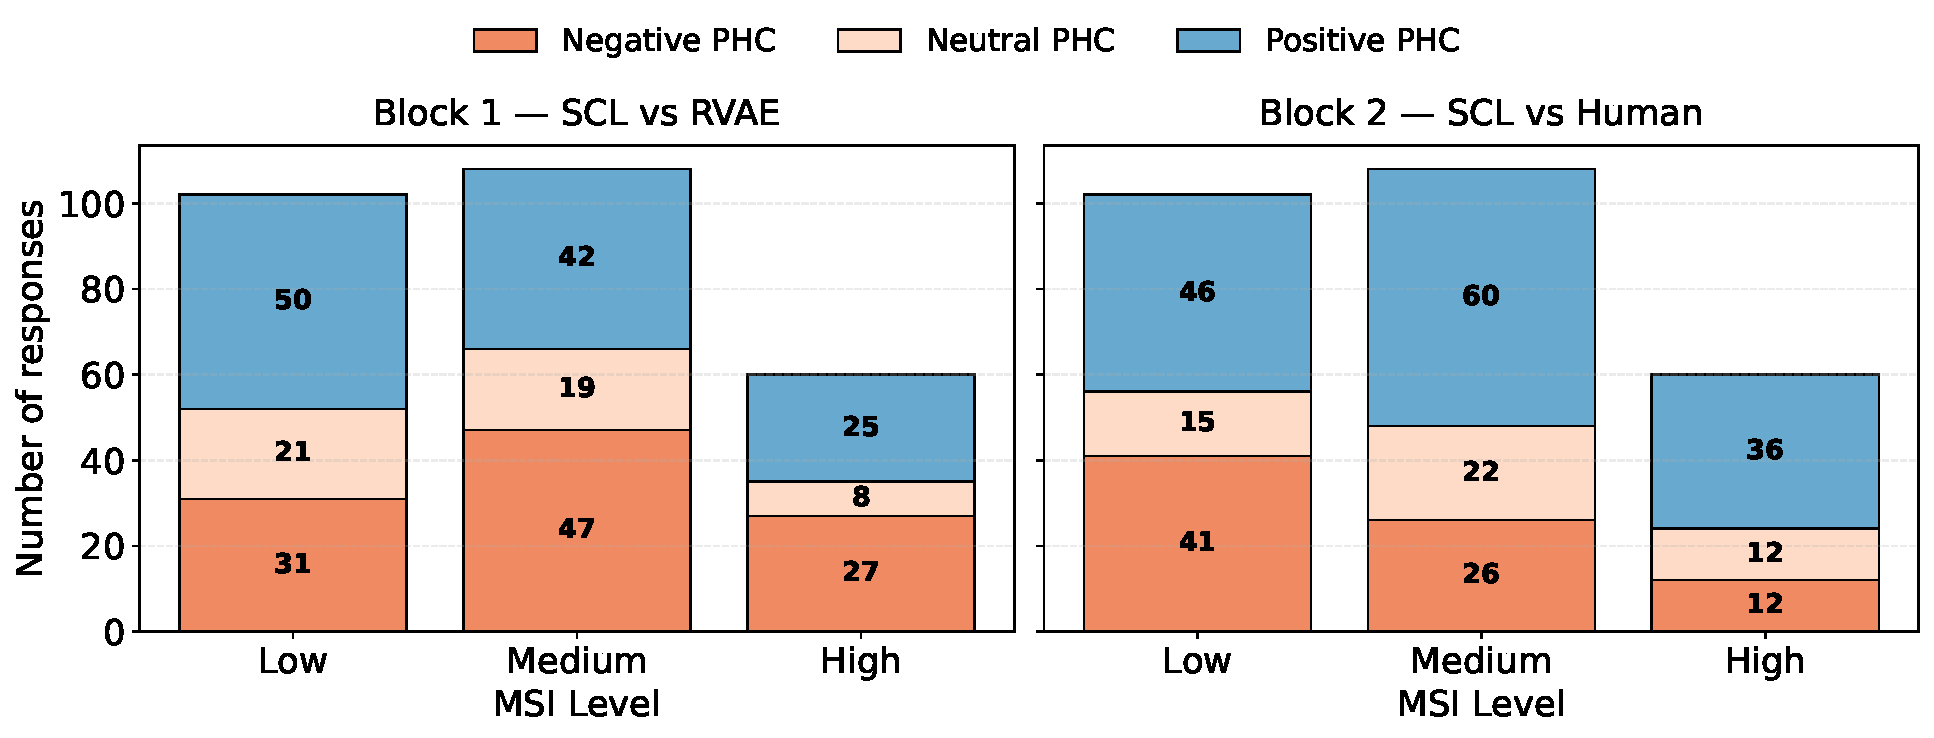
\includegraphics[width=0.5\textwidth]{img/phc.pdf}
\caption{Distribution of PHC response types grouped by musical training level (MTS) and experimental block conditions.}
\label{fig:form_stats}
\end{figure}
\subsection{Subjective Evaluation Results}

A total of 53 participants completed the listening test. After applying two control questions as filters, 45 participants were retained for analysis. Figure~\ref{fig:form_stats} shows the distribution of PHC response types by musical training level (Low, Medium, High) across the experimental blocks.
Table~\ref{tab:phc_block1_audio} reports PHC values for each audio fragment in Block 1 (SCL vs RVAE), ranging from -0.422 to 0.556. The majority of fragments (4 of 6) exhibit positive PHC, though with high inter-participant variability (SD $>$ 1.0 in all cases), suggesting a trend toward SCL being perceived as more complex than RVAE, but with considerable listener disagreement. 
Analyzing the SCL outputs, progressions including chromatic shifts or extended harmonies (such as Cmin–F$\sharp$min–A7–D$\sharp$min–Cmin and Am–Bm7$\flat$5–Em7–Am7), appeared with relatively large positive or negative PHC values. However, sequences with lower harmonic variation or more diatonic motion (such as Cm–B$\flat$–B$\flat$–Dm7–E$\flat$ and Am–G–F–G), were generally associated with moderate or negative values.
Predominantly positive PHC values indicate that SCL-generated progressions were generally perceived as more harmonically complex than RVAE outputs.
Average PHC was higher for Low MTS participants (0.245 $\pm$ 0.670) than for Medium (-0.065 $\pm$ 0.746) and High (0.033 $\pm$ 0.838), consistent with the larger number of positive responses observed in the Low MTS group (50 positives vs. 31 negatives), while Medium and High MTS groups showed more balanced responses (Figure~\ref{fig:form_stats}).

\begin{table}[t]
\centering
\caption{PHC values per audio fragment in Block 1 with corresponding SCL-generated chord progressions.}
\label{tab:phc_block1_audio}
\resizebox{\columnwidth}{!}{
\begin{tabular}{l p{6.5cm} c}
\hline
\textbf{Audio} & \textbf{SCL Progression} & \textbf{PHC$_1$} \\
\hline

A\_L2 & 
Cmin – Gmaj – C7 – Fmin – Cmin 
& 0.02 $\pm$ 1.20 \\

A\_L4 & 
Cmin – Gmaj – F$\sharp$7 – F7 – Cmin 
& 0.11 $\pm$ 1.15 \\

A\_L6 & 
Cmin – F$\sharp$min – A7 – D$\sharp$min – Cmin 
& -0.42 $\pm$ 1.31 \\

B\_L1 & 
Cm – B$\flat$ – A$\flat$ – C$\sharp$ – E$\flat$ 
& 0.29 $\pm$ 1.31 \\

B\_L3 & 
Cm – B$\flat$ – B$\flat$ – Dm7 – E$\flat$ 
& -0.11 $\pm$ 1.35 \\

B\_L5 & 
Cm – B$\flat$ – B$\flat$ – Cm7 – Fm7 
& 0.56 $\pm$ 1.22 \\

\hline
\end{tabular}
}
\end{table}

Table~\ref{tab:phc_block2_audio} reports PHC values for Block 2 (SCL vs human reharmonizations). Most fragments show positive values (range -0.200 to 0.933), though with substantial inter-participant variability (SD $>$ 1.0 in all cases). Average PHC increased with MTS level (Low: 0.088 $\pm$ 0.759; Medium: 0.509 $\pm$ 0.638; High: 0.650 $\pm$ 0.709), consistent with the higher number of positive responses observed in Medium and High MTS groups (60 and 36 positives, respectively), while the Low MTS group showed greater response variability (Figure~\ref{fig:form_stats}).
\begin{table}[t]
\centering
\caption{PHC values per audio fragment in Block 2 with corresponding SCL-generated chord progressions.}
\label{tab:phc_block2_audio}
\resizebox{\columnwidth}{!}{
\begin{tabular}{l p{6.5cm} c}
\hline
\textbf{Audio} & \textbf{SCL Progression} & \textbf{PHC$_2$} \\
\hline

A\_H2 &
Dm – B$\flat$7 – Am9 – E$\flat$ – Dm9 – G7 – Amaj7
& 0.31 $\pm$ 1.26 \\

A\_H4 &
G – F – G
& 0.40 $\pm$ 1.07 \\

A\_H6 &
Am – G – F – G
& -0.20 $\pm$ 1.14 \\

B\_H1 &
Fmaj9 – Em7 – D – Dm
& 0.04 $\pm$ 1.40 \\

B\_H3 &
Dm9 – Em7 – Dm7 – Em7
& 0.93 $\pm$ 1.25 \\

B\_H5 &
Am – Bm7$\flat$5 – Em7 – Am7
& 0.80 $\pm$ 1.38 \\

\hline
\end{tabular}
}
\end{table}
\subsection{Objective Evaluation Results}
Table~\ref{tab:objective_results_block2_models_combined} shows objective harmonic complexity metrics for simple progressions, human reharmonizations, RVAE, and SCL. Overall, human reharmonizations generally present higher dissonance and chord complexity (VT, VS, VDR, 7C, NSC, CC) compared to simple progressions. RVAE and SCL show intermediate values in dissonance (VT, VDR) and variability (VNSPC). Standard triads (ST) decrease in human and partially in RVAE progressions. PRTMCVI reflects differences in interval distribution across models.


To verify that higher complexity scores do not trivially result from unrelated or random chord sequences, we include a Random baseline (chords drawn uniformly from the vocabulary, matching input length) in Table~\ref{tab:objective_results_block2_models_combined}. The Random baseline achieves the highest scores on most complexity metrics, confirming that complexity alone is not a sufficient evaluation criterion. To complement these metrics, we measure input--output relatedness as defined in Section~\ref{sec:objetive}. Table~\ref{tab:objective_results_block2_models_combined} reports relatedness across all conditions: SCL Default achieves 0.566, SCL Tuned ($\tau$=1.26, $N$=19) achieves 0.513, human reharmonizations achieve 0.683, RVAE achieves 0.377, the Simple baseline achieves 1.0 by construction, and the Random baseline achieves approximately zero. These results indicate that while SCL increases harmonic complexity relative to simple inputs, it does so with a measurable degree of input--output relatedness, and notably outperforms RVAE (0.566 vs 0.377) in preserving structural connection to the original progression.


About CHCS, table \ref{tab:chcs_results} summarizes the obtained results. Human reharmonizations generally exhibit the highest CHCS, particularly when chord diversity is prioritized. The SCL model generally achieves higher CHCS values than RVAE across most configurations, occasionally exceeding the human baseline in dissonance- or distribution-focused settings. RVAE shows moderate increases over simple progressions but rarely reaches the levels of human or SCL-generated sequences.
\subsection{Discussion}

Comparing subjective ratings (PHC) with objective CHCS metrics, human reharmonizations achieve the highest CHCS values but were not always perceived as the most complex. SCL-generated progressions show elevated values in dissonance and interval distribution, outperforming RVAE outputs and approaching the values observed in human reharmonizations. Notably, SCL also achieves substantially higher input--output relatedness than RVAE (0.566 vs 0.377), indicating that the music-theoretic losses guide the model toward musically meaningful transformations rather than arbitrary complexity increases. This pattern holds across hyperparameter settings, with SCL Tuned ($\tau$=1.26) reaching 0.513, still well above RVAE's score. However, the perceptual impact varies across fragments: some progressions with chromatic shifts (e.g., Cmin--F$\sharp$min--A7--D$\sharp$min--Cmin) received divergent ratings between low and high MTS participants, suggesting that musically trained listeners may be more sensitive to structural coherence beyond raw complexity. In contrast, chord diversity, which contributes to the CHCS of human reharmonizations, is not consistently reflected in PHC trends across fragments. Overall, CHCS provides an aggregated objective measure of harmonic complexity, while PHC reflects the perceptual aspects emphasized by listeners during evaluation.

\subsection{Limitations}
Several aspects of this study suggest directions for further investigation. The dataset covers Western popular music progressions of 4--7 chords, and the model uses a compact architecture (single-layer LSTM, hidden size~64); evaluating SCL on larger corpora and longer sequences would test its generalization capacity. The listening test focused on perceived harmonic complexity; future studies could complement this with additional perceptual dimensions such as coherence and aesthetic preference. The input--output relatedness metrics presented here were computed on a set of six paired progressions; extending this analysis to a larger and more diverse sample would strengthen the characterization of the enrichment process. Finally, while the training dynamics indicate that all music-theoretic loss terms contribute stably during learning, a systematic ablation of individual terms would quantify their specific impact on the generated outputs.


\begin{table}[t]
\centering
\caption{Objective CHCS evaluation results.}
\label{tab:chcs_results}
\resizebox{0.9\columnwidth}{!}{
\footnotesize
\begin{tabular}{lccc}
\hline
\textbf{Weight Configuration} & \textbf{Human} & \textbf{RVAE} & \textbf{SCL Default} \\
\hline
More Dissonance                 & 0.657 & 0.456 & 0.590 \\
More Chord Diversity            & 0.672 & 0.497 & 0.501 \\
More Distribution               & 0.652 & 0.502 & 0.584 \\
Balanced                        & 0.657 & 0.481 & 0.574 \\
Highly Dissonance-Focused       & 0.646 & 0.429 & 0.656 \\
Highly Chord Diversity-Focused  & 0.692 & 0.500 & 0.417 \\
Highly Distribution-Focused     & 0.635 & 0.513 & 0.645 \\
\hline
\end{tabular}
}
\end{table}
\begin{table}[t]
\centering
\caption{Objective CHCS under different harmonic weighting configurations for two SCL generation settings.}
\label{tab:chcs_comparison_filtered}
\resizebox{0.9\columnwidth}{!}{
\footnotesize
\begin{tabular}{lcc}
\hline
\textbf{Weight Configuration} & \textbf{$\tau$1.0\_N5 (SCL Default)} & \textbf{$\tau$1.26\_N19} \\
\hline
More Dissonance                & 0.568 & 0.621 \\
More Chord Diversity           & 0.450 & 0.680 \\
More Distribution              & 0.543 & 0.667 \\
Balanced                       & 0.540 & 0.649 \\
Highly Dissonance-Focused      & 0.655 & 0.581 \\
Highly Chord Diversity-Focused & 0.352 & 0.700 \\
Highly Distribution-Focused    & 0.609 & 0.666 \\
\hline
\end{tabular}
}
\end{table}
\subsection{Hyperparameter sensitivity analysis}
To analyze the effect of hyperparameter variation in SCL, we conducted a tuning process using the tool \texttt{irace}~\cite{LopDubPerStuBir2016irace}. The tuning scenario considered the generation-stage hyperparameters $N$ and $\tau$.
Table~\ref{tab:objective_results_block2_models_combined} reports the results obtained using the default hyperparameter configuration SCL Default ($\tau$1.0\_N5) and the configuration selected by \texttt{irace} ($\tau$1.26\_N19). Table~\ref{tab:chcs_comparison_filtered} presents the corresponding Composite Harmonic Complexity Scores (CHCS) under different weighting configurations. Considering CHCS values under different weighting schemes, the tuned configuration presents higher scores in weightings emphasizing chord diversity and interval distribution, whereas the default configuration presents higher scores under weightings emphasizing dissonance. Balanced weightings yield similar scores between configurations. These results show that hyperparameter selection is associated with differences in the harmonic characteristics of generated progressions, including dissonance-related measures, chord usage, and interval distribution.
\section{Conclusions and Future Work}
\label{sec:conclusions}

This work presents SCL, a semi-supervised VAE-LSTM framework for harmonic enrichment of chord progressions.
The proposed two-phase semi-supervised strategy---combining latent pretraining, supervised enrichment, and differentiable music-theoretic losses---enables harmonic transformations that increase complexity while maintaining measurable input--output relatedness, without requiring melodic guidance.
Objective results show that SCL increases harmonic complexity relative to simple inputs and outperforms RVAE across most metrics. A random chord baseline confirms that complexity alone is insufficient as an evaluation criterion, as it achieves the highest scores on most complexity metrics. The input--output relatedness metrics provide a complementary measure that distinguishes SCL from random generation. Subjective evaluations reveal that listeners with higher musical training are more sensitive to structural coherence in generated outputs, highlighting the importance of perceptual quality alongside objective complexity. Future work includes evaluating SCL across additional musical styles, incorporating perceptual quality measures, conducting ablation studies on individual loss terms, and scaling the architecture to larger datasets and longer progressions.


{\small
\bibliographystyle{IEEEtran}
\bibliography{references}
}

% For non BibTeX users:
%\begin{thebibliography}{citations}
% \bibitem{Author:17}
% E.~Author and B.~Authour, ``The title of the conference paper,'' in {\em Proc.
% of the Int. Society for Music Information Retrieval Conf.}, (Suzhou, China),
% pp.~111--117, 2017.
%
% \bibitem{Someone:10}
% A.~Someone, B.~Someone, and C.~Someone, ``The title of the journal paper,''
%  {\em Journal of New Music Research}, vol.~A, pp.~111--222, September 2010.
%
% \bibitem{Person:20}
% O.~Person, {\em Title of the Book}.
% \newblock Montr\'{e}al, Canada: McGill-Queen's University Press, 2021.
%
% \bibitem{Person:09}
% F.~Person and S.~Person, ``Title of a chapter this book,'' in {\em A Book
% Containing Delightful Chapters} (A.~G. Editor, ed.), pp.~58--102, Tokyo,
% Japan: The Publisher, 2009.
%
%\end{thebibliography}

\end{document}